\chapter{Theory of neutrino physics}\label{sec:NeutrinoTheory}
%%%%%%%%%%%%%%%%%%%%%%%%%%%%%%%%%%%%%%%%%%%%%%%%%%%%%%%%%%%%%%%%%%%%%%%%%%%%%%%
%%% 1. Brief history up to neutrinos being in the SM

Neutrinos were first introduced by Wolfgang Pauli \cite{PauliNeutrinoProposalLetter.pdf,TheIdeaOfTheNeutrino.pdf} as very light electrically neutral particles with half-spin and a possible magnetic moment \cite{NeutrinoMagMomentImplications1934.pdf}. They were a crucial part of Enrico Fermi's successful theory of $\beta$ decays \cite{FermisTheoryOfBetaDecayOriginal.pdf, FermisTheoryOfBetaDecay.pdf}, which solidified their importance in particle physics even before their first experimental detection.
Fermi's theory developed into the \gls{SM} of particle physics \cite{SMGlashow.pdf,SMWeinberg.pdf,SMSalam.pdf}, which in its current form contains three generations of fermions. Each generations contains two quarks, one charged lepton and an associated neutrino with no mass or magnetic moment. 

\gls{SM} is mathematically described by a Lagrangian, in which neutrinos are expressed as two-component left-handed chiral fields $\nu_{\alpha L}$, where $\alpha=e,\mu,\tau$ denotes the three neutrino generations, also called flavours \cite{LandauParityViolationForNus.pdf, LeeYangNuAsMasslessWeylSpinor.pdf, SalamNuAsMasslessWeylSpinors.pdf}. Neutrinos form weak isospin doublets with their associated left handed charged lepton fields $\alpha_L$. Unlike for the charged leptons, there is no right handed neutrino singlet in the \gls{SM}. This means that neutrinos cannot obtain a (Dirac) mass term, since the mass terms for fermions arise from the Higgs mechanism \cite{HiggsMechanismOriginal1964.pdf, HiggMechanismEnglertBrut1964.pdf, HiggsMechanismGuralnikHagenKibble1964.pdf} via the Yukawa coupling of the fermion and the Higgs fields \cite{YukawaLagrangiaWeinberg1967.pdf}, which requires a combination of left-handed and right-handed fields \cite{FundamentalsOfNeutrinoPhysics.pdf}.

\todo{Mention that antineutrinos in the SM are right handed and therefore related to neutrinos via CP symmetry}
%\cite{FundamentalsOfNeutrinoPhysics.pdf} Physical neutrinos and antineutrinos are related by a CP transformation which interchanges neutrinos with antineutrinos and reverses helicity: $\nu\longleftrightarrow\overline{\nu}$ with CP (in the case of Majorana neutrinos, where the C transformation coincides with the identity, it is conventional to call neutrinos the states with negative helicity and antineutrinos the states with positive helicity)

%\cite{FundamentalsOfNeutrinoPhysics.pdf} In the SM, the mass of fermions arises as a result of the Higgs mechanism through the presence of Yukawa couplings of the fermion fields with the Higgs doublet. ... a fermion mass term must involve a coupling of left-handed and right-handed fileds, so it is clear that in the SM neutrinos are massless, because their fields do not have a right-handed components

The interaction terms for neutrinos can be separated into two parts, describing the \gls{CC} and the \gls{NC} interactions, based on whether they interact with the $W_\mu$ or $Z_\mu$ massive gauge fields, which describe the $W^\pm$ or $Z^0$ weak boson respectively. Neglecting the non-neutrino components, the two neutrinos interaction terms are \cite{FundamentalsOfNeutrinoPhysics.pdf}
\begin{equation}\label{eq:NuIntLagrangian}
\mathcal{L}_{\textsc{CC}}^{\textsc{SM}}=-\frac{g_w}{2\sqrt{2}}j^\mu_W W_\mu +\textsf{h.c.},\,\,\,\textsf{and}\,\,\,
\mathcal{L}_{\textsc{NC}}^{\textsc{SM}}=-\frac{g_w}{2\cos\left(\theta_W\right)}j^\mu_Z Z_\mu.
\end{equation}
Here $g_w$ is the weak coupling constant, $\theta_W$ is the Weinberg angle and $j^\mu_W$ and $j^\mu_Z$ are the weak currents expressed as
\begin{equation}\label{eq:NuIntCCCurrent}
j^\mu_W=2\sum_{\alpha=e,\mu,\tau}\overline{\nu}_{\alpha L}\gamma^\mu\alpha_L,
\end{equation}
\begin{equation}\label{eq:NuIntNCCurrent}
j^\mu_Z=\sum_{\alpha=e,\mu,\tau} \overline{\nu}_{\alpha L} \gamma^\mu \nu_{\alpha L},
\end{equation}
where $\gamma^\mu,\mu=0,1,2,3$, are the four Dirac gamma matrices.

The two terms of the interaction Lagrangian from Eq.~\ref{eq:NuIntLagrangian} describe the possible neutrino interaction vertices shown in Fig.~\ref{fig:FeynmanNuIntVertices}. These diagrams show the \gls{CC} and the \gls{NC} interaction of neutrinos and antineutrinos and, in case of the \gls{CC} diagram, can also be flipped around the vertical axis to show the production of neutrinos from the weak interaction (or decays) of leptons. They can also be rotated $90^{\circ}$ to either show the annihilation, or the production of the neutrino-lepton (for \gls{CC}), or neutrino-antineutrino (for \gls{NC}) pairs.

\begin{figure}[hbtp]
\centering
%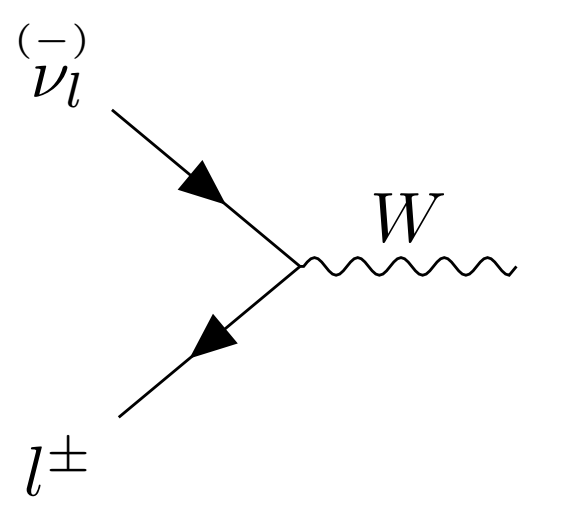
\includegraphics[height=3.2cm]{Plots/Theory/NeutrinoCCAnnihilationVertices.png}
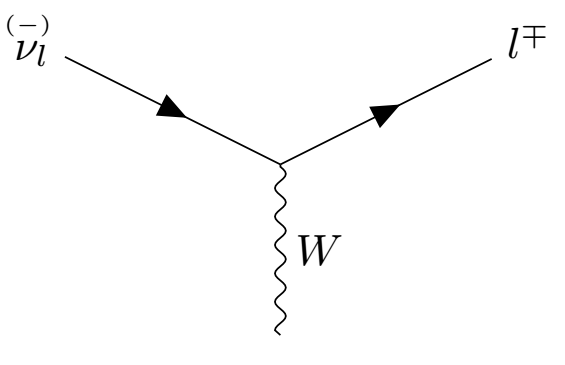
\includegraphics[width=.4\linewidth]{Plots/Theory/NeutrinoCCInteractionVertices.png}
\hspace{0.1\linewidth}
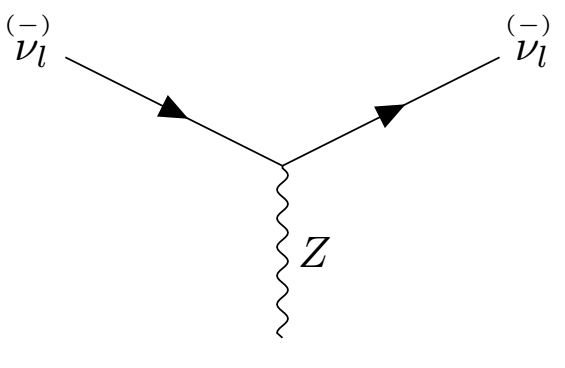
\includegraphics[width=.4\linewidth]{Plots/Theory/NeutrinoNCInteractionVertices.png}
\caption[Neutrino interaction vertices in the SM]{Neutrino interaction vertices in the \acrshort{SM} via the weak charged currents (left) and the neutral currents (right).}
\label{fig:FeynmanNuIntVertices}
\end{figure}


% in weak isospin doublets \cite{FundamentalsOfNeutrinoPhysics.pdf} grouped with their lepton left handed chiral components of charge leptons. Since SM neutrinos do not have a right handed counterpart, they can't acquire mass through the Yukawa lagrangian which combined the left and right handed fields. Their interaction lagrangian is...

%Neutrinos in the \gls{SM} are described as massless with a left-handed chiral field, with no right-handed neutrino chiral field counter part. Neutrinos make a lepton doublet together with their associated leptons. There are no neutrino mass terms in the \gls{SM} Lagrangian and the interaction terms can be divided into two types: the \gls{CC} and the \gls{NC} interactions \cite{FundamentalsOfNeutrinoPhysics.pdf}

%Neutrinos are grouped together with their corresponding charged lepton to form isospin doublets with no right handed neutrino singlet counterpart. In the SM a fermion mass term must involve a coupling of left-handed and right-handed fields and since neutrinos only have left handed fields they can't obtain

%[nuMM/nuElmagInt2015.pdf] However, there was no sign of a neutrino mass. After the discovery of parity violation in 1957, Landau (1957), Lee and Yang (1957), and Salam (1957) proposed the two-component theory of massless neutrinos, in which a neutrino is described by a Weyl spinor and there are only left-handed neutrinos and right-handed antineutrinos. It was, however, clear (Case, 1957; Mclennan, 1957; Radicati and Touschek, 1957) that two-component neutrinos could be massive Majorana fermions and that the two-component theory of a massless neutrino is equivalent to the Majorana theory in the limit of zero neutrino mass. The two-component theory of massless neutrinos was later incorporated in the standard model of Glashow (1961), Weinberg (1967), and Salam (1969), in which neutrinos are massless and have only weak interactions. In the standard model Majorana neutrino masses are forbidden by the $\textsf{SU}\left(2\right)_L\times \textsf{U}\left(1\right)_{\gamma}$ symmetry.

%[nuMM/nuElmagInt2015.pdf] In the standard model of electroweak interactions (Glashow, 1961; Weinberg, 1967; Salam, 1969), neutrinos are described by two-component massless left-handed Weyl spinors (Giunti and Kim, 2007). The masslessness of neutrinos is due to the absence of right-handed neutrino fields, without which it is not possible to have Dirac mass terms, and to the absence of Higgs triplets, without which it is not possible to have Majorana mass terms.

%[OverviewOfNeutrinoPhysicsPheno2024.pdf] three neutrino flavours produced with charged antilepton, or producing a charged lepton in CC weak interaction processes. Therefore neutrino have exhibited a polarisation in a direction that is opposite to their motion, or, equivalently, with negative helicity. For antineutrino it is the opposite. To account for this neutrino are described in the SM with a left handed chiral field $\nu_{\alpha L}\left(x\right)$. In the absence of neutrino masses, this field destroys (creates) neutrinos (antineutrinos) with negative (positive) helicity.  In the SM, neutrinos are considered massless, and no right-handed (RH) neutrino chiral field is included in its content as they would be singlet under the SM gauge group. As such, the corresponding RH neutrinos would be completely inert. Neutrinos and their lepton LH fields form SU(2) doublets $\psi_{\alpha L}\left(x\right)=\left(\nu_{\alpha L}\left(x\right),\alpha_L\left(x\right)\right)$ with hypercharge +1.

%%%%%%%%%%%%%%%%%%%%%%%%%%%%%%%%%%%%%%%%%%%%%%%%%%%%%%%%%%%%%%%%%%%%%%%%%%%%%%%
%%% 2. Neutrino production and sources
\section{Neutrino Production}
Some of the most common neutrino and antineutrino production channels include nucleon transitions via \gls{CC} weak interactions. Specifically, the transition of a neutron into a proton, either as a decay of a free neutron, or as a $\beta^-$ decay for neutrons bound in a nucleus, produces an electron and an electron antineutrino:
\begin{equation}
n\rightarrow p+e^-+\overline{\nu}_e.
\end{equation}
The study of the shape of the electron spectrum from $\beta^-$ decay was the reason Pauli proposed the existence of the neutrino \cite{PauliNeutrinoProposalLetter.pdf}. Additionally, this channel is an abundant source of $\overline{\nu}_e$ from nuclear reactors, which were the first artificial sources of neutrinos, increasing the neutrino flux by about 100 million compared to the naturally occurring sources, enabling the first ever detection of a neutrino \cite{CowanReinesFirstAttempt.pdf, CowanReinesConfirmation.pdf, NeutrinoPhysicsCowanReines.pdf}.

Similarly, the production of an electron neutrino via the transition of a proton into a neutron can occur inside the nucleus either as the $\beta^+$ decay:
\begin{equation}
p\rightarrow n+e^++\nu_e,
\end{equation}
or via the electron capture:
\begin{equation}
p+e^-\rightarrow n+\nu_e.
\end{equation}
This channel occurs in stars and in the first phase of supernovae \cite{FundamentalsOfNeutrinoPhysics.pdf}.

However, most supernovae neutrinos are created via a thermal pair production via \gls{NC} interaction
\begin{equation}
e^-+e^+\rightarrow\nu_\alpha+\overline{\nu}_\alpha
\end{equation}
producing neutrinos and antineutrinos of all flavours. Neutrino pair production via the decay of $Z^0$ was studied in great detail \cite{ZDecay.pdf}, since the magnitude of the decay width depends on the number of light active neutrino flavours, with the current best fit $N_\nu=2.984$ \cite{ZDecayPrecise.pdf}.
%Similar interactions produced the currently unobservable relic neutrinos, which were produced during the Big Bang and have extremely low energies.

%In 1990 the L3 Collaboration studied properties of the $Z^0$ boson and fitted to its peak cross-section and decay width to determine the total number of active (interacting with $Z^0$) light ($m_{\nu}<m_{Z}/2$) neutrino flavours ($N_{\nu}$). They found the best fit integer value to be 3 and ruled out the possibility of four or more active light neutrino flavours at $4\sigma$ \cite{ZDecay.pdf}. Latest most precise results put the fitted value to $N_{\nu}=2.9840\pm 0.0082$ \cite{ZDecayPrecise.pdf}.

An abundant source of $\nu_\mu$ and $\overline{\nu}_\mu$ is the decay of pions and muons
\begin{align}
p+X \rightarrow \pi^\pm \rightarrow &\mu^\pm + \nu_\mu\left(\overline{\nu}_\mu\right) \\
 & \mu^\pm \rightarrow e^\pm + \nu_\mu\left(\overline{\nu}_\mu\right) + \nu_e\left(\overline{\nu}_e\right),
\end{align}
which naturally occurs in Earth's atmosphere from the interaction of cosmic ray protons. It is notable, that if all the muons decay by the time they reach Earth's surface, the ratio of $\nu_\mu : \nu_e$ should be exactly 2:1. This processed is also used in the modern accelerator-based sources of neutrinos, which accelerate protons to the desired energies, impinge them onto a fixed target, and focus the resulting hadrons to achieve a highly pure and precise source of $\nu_\mu$ or $\overline{\nu}_\mu$ \cite{GoodmanAdvancesInNeutrinoPhysics.pdf, SchwartzAccelerators.pdf}. Similarly, decays of heavier hadrons, such as kaons and charmed particles, also produce neutrinos, including $\nu_\tau$ and $\overline{\nu}_\tau$ \cite{ObservationOfTauNeutrino.pdf, FinalTauNeutrinoResultsDONUT2008.pdf}.

%[Master's] The advent of fission reactors brought increase of neutrino rate of about $10^7$, as well as higher neutrino energies, making the neutrino detection worth reinvestigating \cite{NeutrinoPhysicsCowanReines.pdf}. In 1960 Mel Schwartz designed the first neutrino beam made by accelerated protons striking a target, producing pions (mostly), which would decay into neutrinos \cite{GoodmanAdvancesInNeutrinoPhysics.pdf}\cite{SchwartzAccelerators.pdf}.

%%%%%%%%%%%%%%%%%%%%%%%%%%%%%%%%%%%%%%%%%%%%%%%%%%%%%%%%%%%%%%%%%%%%%%%%%%%%%%%
%%% 3. Interaction of neutrinos
\section{Neutrino Interactions}
The interaction of neutrinos can either be categorized based on the target, which is generally either electron or a nucleus, or on the neutrino energy.

Neutrino-electron interactions occur either via elastic scattering, which result in a neutrino and an electron in the final state, or via the inverse muon (or tau) decay, which contains a muon (or tau) in the final state. Both of these interactions are purely governed by \gls{QED} and are theoretically very well understood, and we are currently using their measurements to provide constraints on the parameters within the \gls{QED} theory. Additionally, while the neutrino-on-electron elastic scattering does not have a threshold energy and can occur for any neutrinos, the inverse muon decay has a threshold for the $\nu_\mu$ energy of $\unit[10.92]{GeV}$, and the inverse tau decay $E_{\nu_\tau}>\unit[3]{TeV}$ \cite{FundamentalsOfNeutrinoPhysics.pdf, NeutrinoOnElectronElScatteringTheory2003.pdf}.

%Interaction with nucleons
%By increasing their energy, neutrinos can interact with the individual nucleons bound inside the nucleus above a certain threshold \note{But this threshold doesn't really exist tbh} we can start describing the nucleus as a collection of individual, quasi-free nucleons and we can consider interaction of neutrinos on free nucleons \cite{NeutrinoIntOverview2012.pdf}. 

The interaction of neutrinos with a nucleus can be to an extent approximated by an interaction of neutrinos on quasi-free nucleons \cite{NeutrinoIntOverview2012.pdf}. The interaction of neutrinos on nucleons can be further classified based on the products it generates. We illustrate these categories on a case of $\nu_\mu$ \gls{CC} cross section in Fig.~\ref{fig:NuCCCrossSection}. At lower energies neutrinos interact via the elastic interactions in the \gls{NC} channel, simply kicking the nucleon out of the nucleus, and via the \gls{QE} interactions in the \gls{CC} channel, transforming the neutron or proton into its nucleon counterpart. For example, the \gls{QE} interaction of an antineutrino on a proton
\begin{equation}
\overline{\nu}_l +p\rightarrow n+l^+
\end{equation}
is often called the inverse $\beta$ decay and it was used for the first ever detection of neutrinos (specifically electron antineutrinos from a nuclear reactor) by Cowan and Reines \cite{CowanReinesFirstAttempt.pdf, CowanReinesConfirmation.pdf}. Analogically, the interaction of neutrinos on a neutron
\begin{equation}
\nu_l+n\rightarrow p+l^-
\end{equation}
is interesting especially due to having no low energy threshold for $\nu_e$ and it is commonly used for detection of solar neutrinos \cite{Homestake1968.pdf}. For $\nu_\mu$ and $\nu_\tau$ there is a low energy threshold for the \gls{QE} interactions on a free nucleon. For $\nu_\mu$ this threshold is about $\unit[110]{GeV}$, which can be clearly seen in Fig.~\ref{fig:NuCCCrossSection} as the drop off cross section at low energies. The $\nu_\mu$ \gls{CC}\gls{QE} channel was used for the first detection of $\nu_\mu$ \cite{MuonNeutrinoDetection.pdf} from an accelerator and is commonly used for the detection of atmospheric neutrinos \cite{FirstAtmosphericNuDetIndia.pdf, FirstAtmosphericNuDetIndia2.pdf, FirstAtmNuDetectionSouthAfrica1965.pdf}. The threshold for the \gls{CC}\gls{QE} interaction of $\nu_\tau$ is about $\unit[3.5]{GEV}$, which meant that it was only discovered only in 2000 by the DONUT Collaboration at Fermilab \cite{ObservationOfTauNeutrino.pdf}.

\begin{figure}[hbtp]
\centering
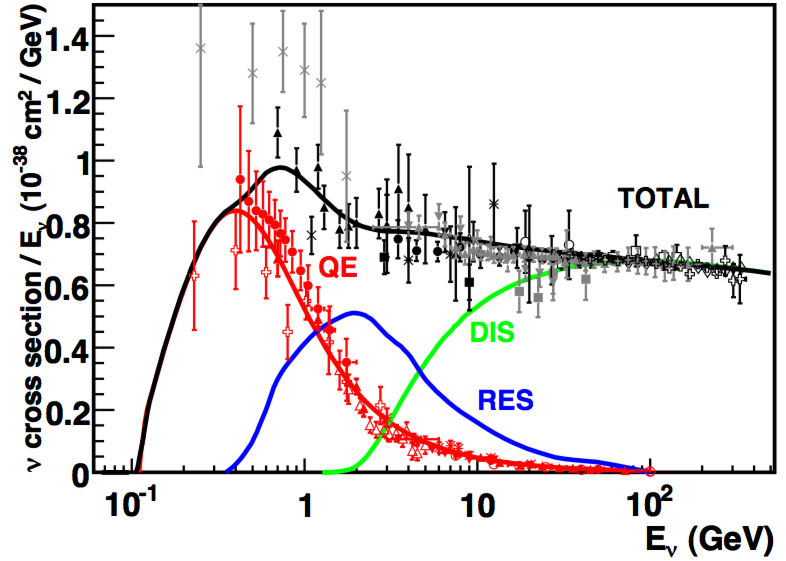
\includegraphics[width=0.8\linewidth]{Plots/Theory/NeutrinoCCCrossSections.png}
\caption[Muon neutrino CC cross sections based on the interaction types]{Neutrino \acrshort{CC} cross sections on an isolated nucleon divided by the neutrino energy based on the interaction types. Figure is from \cite{NeutrinoCCCrossSectionPlot.pdf} and compares the measured data \cite{NeutrinoIntOverview2012.pdf} and the prediction provided by the NUANCE generator \cite{NuanceNuIntSimulation2002.pdf}.}
\label{fig:NuCCCrossSection}
\end{figure}

%%% Resonance production and DIS
With an increase in neutrino energy above a certain threshold (about $\unit[270]{MeV}$ for $\nu_\mu$), neutrinos start the \gls{Res}, which commonly decay into a nucleon and an additional hadron. These hadrons are initially pions at lower energies, but by increasing the neutrino incident energy, they start producing multiple pions and other mesons and hyperons. With even higher incident energies, neutrinos start probing the quark contents of the individual nucleons in the \gls{DIS} interaction, as can be seen in Fig.~\ref{fig:NuCCCrossSection}.

%Mention that the NC resonance production of $\pi^0$ or $\gamma$ could potentially mimic the electron signal so this can be a significant background for the nuone interactions. In the case for resonant production neutrino produces an additional hadron to the nucleon from the QE interactions...

%[NeutrinoIntForLBL2016.pdf] At energies above $\approx \unit[200]{MeV}$, the first inelastic excitations of the nucleon connected with pion production become possible. The threshold is $\unit[150.5]{MeV}$ for $\nu_e$ and $\unit[277.4]{MeV}$ for the $\nu_\mu$

%With higher energies there can be more pions and also other mesons or hyperons and so on.

%For DIS the neutrino doesn't interact with the nucleon as a whole but with its quark constituents

%%% Nuclear effects
Even though the approximation of nuclei as collections of quasi-free nucleons is useful, it has been shown \cite{MiniBooNE2p2hExperimentalDiscrepancy2010.pdf} that there are important nuclear effects that have to be considered. Example of these are: Fermi motion of nucleons and their binding inside the nucleus,  Pauli's exclusion principle and nucleon energy levels, short and long range nucleon-nucleon correlations, \gls{MEC}, or \gls{FSI} \cite{NeutrinoIntOverview2022.pdf}.

Additionally, if the total energy transferred to the nucleus is small relative to the size of the nucleus, neutrinos can interact with the entire nucleus coherently. At low energies, neutrinos can interact via the \gls{CEvNS}, where the contributions from each individual nucleon are simply added together coherently \cite{CEvENSFirstObservation2017.pdf}, leaving behind an excited nucleus. At higher energies, neutrinos can interact via the \gls{COHpi} without transferring much momentum to the nucleus. Therefore, there is only a single pion produced (charged through \gls{CC}\gls{COHpi} and neutral through \gls{NC}\gls{COHpi}), which receives most of the transferred momentum and generally travels in the direction of the initial neutrino. This means that the \gls{COHpi} can mimic real $\mu^\pm$, $e^-$, or $\gamma$ signal in a detector \cite{NeutrinoIntOverview2022.pdf}.

%\cite{NeutrinoIntOverview2022.pdf} Also coherent meson production, in which neutrino scatters from the nucleus producing mesons but the nucleus stays in the ground state, possible via both CC and NC. The momentum transferred to the nuclear target is very small and almost all the transferred momentum is taken by the outgoing meson. The coherence condition $Q\ll 1/R$ is satisfied and the individual amplitudes for the pion production from each nucleon in the nucleus add coherently. Most of the $\pi^\pm,\pi^0$ produced (through the electromagnetic shower as their decay products) in the forward direction through the coherent reactions mimic the real $\mu^\pm$ or $e^-$ signal.

%However, recently we discovered that nuclear effect can't actually be ignored and we can't really consider neutrino nucleus interaction as a neutrino on nucleon interaction. 
Another notable example is the \gls{2p2h} interaction \cite{FirstUseOfMEC2009.pdf, FirstUseOfMEC2010.pdf, FirstUseOfMEC2011.pdf}, which occurs when neutrinos interact with a correlated pair of nucleons, resulting in two nucleons leaving the nucleus, which now has two holes. This interaction can significantly increase the \gls{QE} cross section \cite{NeutrinoIntOverview2022.pdf}. Most frequently, this interaction occurs via the \gls{MEC}, where the meson effectively propagates the interaction between the two bound nucleons.
%[Maria's thesis] A neutrino can interact with a pair of bound nuclei, thus knocking out two nucleons instead of one, as pictured in Figure 1.14. This is also referred as 2p2h, as the interaction leaves two holes in the struck nucleus. Most frequently, this occurs via the meson exchange current (MEC), where the two nucleons are interacting with each other via a meson.

The products of each of the aforementioned interactions can re-interact inside the nucleus in the so-called \gls{FSI}. The final products of the interaction will therefore make it appear as a different interaction inside the detector.
%[Maria's thesis] The nucleons and pions and others particles can re-interact within the nucleus. Specifically for pions there are a number of processes that can happen: absorption, (quasi)elastic scattering, charge exchange,... These can also happen multiple times

%For neutrinos interacting on the nuclei, we distinguish between different types of interactions based on what happens to the nucleus. If it's an interaction with a single proton or neutron, we call this \gls{QE} interaction. If this proton gets excited into a $\Delta$ resonance (which then generally decays into a $\pi$), we call this Resonant production, if neutrino penetrates through the nucleon and interacts directly with a quark inside it, we call this \gls{DIS} interaction. This is shown on Fig.~\ref{fig:NuCCCrossSection}. There can be additional subtypes due to nuclear effects, namely the 2p2h interaction \todo{Find a reference for the 2p2h} also called \gls{MEC}, or possible \gls{FSI}.

%nu-on-e is for example used for the detection of solar neutrinos in the Kamiokande experiments
%Nu-on-e is mainly sensitive to electron neutrinos, whose cross section is about 6 times larger than for the muon/tau neutrinos.

%%%%%%%%%%%%%%%%%%%%%%%%%%%%%%%%%%%%%%%%%%%%%%%%%%%%%%%%%%%%%%%%%%%%%%%%%%%%%%%
%%% Masters
%%% Experimental evidence for neutrino %%%
%Soon after Fermi's description of neutrino interaction, in 1934, Bethe and Peierls realized the possibility of reverting the process of beta decay as a mean of direct detection of the neutrino \cite{BethePeierlsDirectDetection.pdf}. For example an interaction in which incident neutrino interacts with proton, transforming it into neutron and creating a positron. From the lifetime of then-known beta decays they estimated the interaction cross-section to be $<\unit[10^{-44}]{cm^2}$ for a neutrino with a few $\unit{MeV}$ energy, or about $10^{-20}$ times the more familiar nuclear values at the time.

%In 1953 C.~L.~Cowan and F.~Reines placed a liquid scintillation detector near the Hanford reactor reporting uncertain results \cite{CowanReinesFirstAttempt.pdf}. They later moved the detector to the Savannah River Plant and in 1956 confirmed \cite{CowanReinesConfirmation.pdf} the detection of the antineutrino, verifying the neutrino hypothesis \cite{NeutrinoPhysicsCowanReines.pdf}.
%(\ovnu{$\nu$} interacting with proton, producing neutron and positron (\ovnu{$\nu$}$+p\rightarrow n+e^+$))

% Electron neutrino
%The first electron neutrino detection was by the Homestake neutrino experiment detecting solar neutrinos \cite{Homestake1968.pdf}

%%% Muon neutrino %%%
%Leon Lederman, Jack Steinberger and others joined Schwartz and using a spark chamber detector in 1962 observed \cite{MuonNeutrinoDetection.pdf} for the first time the muon neutrino $\nu_{\mu}$. Atmospheric neutrinos were first observed by the Kolar Gold Field Mine in South India \cite{FirstAtmosphericNuDetIndia.pdf, FirstAtmosphericNuDetIndia2.pdf} and in the East Rand Proprietary Gold Mine in South Africa \cite{FirstAtmNuDetectionSouthAfrica1965.pdf}.

% Tau neutrino
%After this result it was only a matter of time, before the third neutrino, the tau neutrino ($\nu_{\tau}$) was discovered. Evidence for that were shown in 2000 from the DONUT Collaboration at Fermilab \cite{ObservationOfTauNeutrino.pdf}.
%%% End of master's on neutrino history
%%%%%%%%%%%%%%%%%%%%%%%%%%%%%%%%%%%%%%%%%%%%%%%%%%%%%%%%%%%%%%%%%%%%%%%%%%%%%%%

%I think I should mention here the basic neutrino interactions and their corresponding cross section. For neutrino on nucleons, the total cross section per neutrino energy is around $\unit[0.7\times 10^{-38}]{cm^2GeV^{-1}}$ for neutrinos and half that for antineutrinos. For neutrino on electron interactions, the total cross section per neutrino energy is more similar to $10^-41-\unit[10^{-42}]{cm^2GeV^{-1}}$.

%Problems of the SM
%[OverviewOfNeutrinoPhysicsPheno2024.pdf] Besides, the SM falls short in describing other challenging issues, including the long-standing problems of explaining the nature of dark matter [12] and the overabundance of matter over antimatter in the Universe [13]. These fundamental problems may be inter-related, with neutrinos potentially playing a primary role in establishing such connections

\section{Neutrino Oscillation}
The idea that neutrinos can oscillate originates as a possible transition between neutrinos and antineutrinos \cite{Pontecorvo57.pdf,Pontecorvo58.pdf}, analogically to the already known oscillations of $K^{0}\leftrightarrow \overline{K^0}$. This was adapted to the oscillations between different neutrino flavours \cite{MNS1962Osc.pdf,Pontecorvo69.pdf} by considering that the flavour neutrino states $\nu_\alpha$, which are the eigenstates of the weak interactions described in Eq.~\ref{eq:NuIntLagrangian}-\ref{eq:NuIntNCCurrent}, are not identical to the mass neutrino states $\nu_k$, which are the eigenstates of the vacuum hamiltonian
\begin{equation}\label{eq:NuOscVacHamiltonian}
\mathcal{H}_0\ket{\nu_k}=E_k\ket{\nu_k}.
\end{equation}

Instead, the neutrino flavour and mass eigenstates are related as
\begin{equation}\label{eq:NuOscFlavourMassRel}
\ket{\nu_{\alpha}}=\sum_{k} U_{\alpha k}^{*}\ket{\nu_{k}},
\end{equation}
where $U$ is the \gls{PMNS} matrix, named after the authors of neutrino oscillations \cite{FundamentalsOfNeutrinoPhysics.pdf, Gonzalez-GarciaNuMassesAndMixing.pdf}. $U$ is defined as unitary, which makes the inverse relation simply
\begin{equation}\label{eq:NuOscMassFlavourRel}
\ket{\nu_k}=\sum_\alpha U_{\alpha k}\ket{\nu_\alpha}.
\end{equation}

From the Schr\"{o}dinger equation
\begin{equation}
i\frac{d}{dt}\ket{\nu_k\left(t\right)}=\mathcal{H}\ket{\nu_k\left(t\right)}
\end{equation}
we get that in vacuum $\left(\mathcal{H}=\mathcal{H}_0\right)$, the massive neutrino states evolve as plane waves
\begin{equation}\label{eq:NuOscPlaneWave}
\ket{\nu_k\left(t\right)}=e^{-iE_kt}\ket{\nu_k},
\end{equation}
where the energy of the neutrino state with mass $m_k$ and momentum $\overrightarrow{p}$ is
\begin{equation}
E_k=\sqrt{\overrightarrow{p}^2+m_k^2}.
\end{equation}
Assuming small neutrinos masses, $E_k$ can be approximated as
\begin{equation}\label{eq:NuOscUltrarelativisticApprox}
E_k\xrightarrow{m^2\ll p^2\approx E^2}E+\frac{m_k^2}{2E}
\end{equation}
for ultra-relativistic neutrinos \cite{FundamentalsOfNeutrinoPhysics.pdf}. Additionally, given the notation $c\equiv 1$,  we can approximate $L\approx t$, where $L$ is the distance neutrino travelled in time $t$ and is easier to measure.

We are interested in the oscillation (transition) of $\nu_\alpha\rightarrow\nu_\beta$ over some experimental baseline $L$. Given that $\braket{\nu_k|\nu_j}=\delta_{kj}$ and $\braket{\nu_{\alpha}|\nu_{\beta}}=\delta_{\alpha\beta}$ and using Eq.~\ref{eq:NuOscPlaneWave},\ref{eq:NuOscFlavourMassRel} and \ref{eq:NuOscMassFlavourRel}, we can write the amplitude of the oscillation as
\begin{equation}
A_{\nu_\alpha\rightarrow\nu_\beta}\left(L\right)\equiv\braket{\nu_\beta|\nu_\alpha\left(L\right)}= \sum_{k} U_{\alpha k}^{*} U_{\beta k} e^{-i E_kL}
\end{equation}
and the probability as
\begin{equation}
P_{\nu_{\alpha}\rightarrow\nu_{\beta}}\left( L\right) =
\left|A_{\nu_\alpha\rightarrow\nu_\beta}\left(L\right)\right|^2 =
\sum_{k, j}U_{\alpha k}^*U_{\beta k}U_{\alpha j}U_{\beta j}^*e^{-i\left(E_k-E_j\right)L}.
\end{equation}

Using Eq.~\ref{eq:NuOscUltrarelativisticApprox} and by defining the neutrino mass splitting (also called the mass squared difference) as
\begin{equation}\label{Deltamsq}
\Delta m_{kj}^{2}\equiv m_{k}^{2}-m_{j}^{2},
\end{equation}
we get
\begin{equation}\label{eq:NuOscProbability}
P_{\nu_{\alpha}\rightarrow\nu_{\beta}}\left( L\right) = \sum_{k, j}U_{\alpha k}^*U_{\beta j}U_{\alpha j}U_{\beta j}^*e^{-i\frac{\Delta m_{kj}^2 L}{2E}}.
\end{equation}

%This led B. Pontecorvo, inspired by already known $K^{0}\leftrightarrow \overline{K^0}$ oscillations, to consider $\nu\leftrightarrow\overline{\nu}$ transitions (oscillations), in case the conservation of neutrino charge does not apply\cite{Pontecorvo57.pdf}. Pontecorvo later built upon this statement in 1958 considering that oscillations between $\nu$ and $\overline{\nu}$ are due to them being combinations of particles $\nu_1$ and $\nu_2$ and that the transformation lifetime is related to the mass difference between $\nu_1$ and $\nu_2$ \cite{Pontecorvo58.pdf}, laying foundation for neutrino oscillations as we know them today.

%In 1962 Z. Maki, M. Nakagawa and S. Sakata applied Pontecorvo's idea of neutrino oscillations to \textit{weak neutrino} eigenstates $\nu_{\alpha}$ ($\nu_e$, $\nu_{\mu}$) produced in weak interactions. They assumed that oscillation $\nu_{\alpha}\leftrightarrow\nu_{\beta}$ are driven by a non-zero mass difference (therefore if true implying at least one neutrino has a non-zero mass) between \textit{true neutrinos} (= mass neutrino eigenstates $\nu_i$ ($\nu_1$, $\nu_2$)), which are related to weak eigenstates via a linear combination. This relation in general case looks like \cite{MNS1962Osc.pdf}
%where $U$ is a unitary matrix now know as Pontecorvo-Maki-Nakagawa-Sakata (PMNS) matrix and $n$ is the (general) number of light neutrino species \cite{Gonzalez-GarciaNuMassesAndMixing.pdf}.

\iffalse
Oscillation probability can be also expressed as
\begin{align}\label{OscProb}
P_{\nu_{\alpha}\rightarrow\nu_{\beta}}\left( L\right)= \delta_{\alpha\beta}
& -4\sum_{i>j}\text{Re} \left( U_{\beta i}U_{\alpha i}^{*} U_{\beta j}^{*}U_{\alpha j}\right)
\sin^{2}\Delta_{ij}\nonumber \\
& +2\sum_{i>j} \text{Im} \left( U_{\beta i}U_{\alpha i}^{*}U_{\beta j}^{*}U_{\alpha j}\right) \sin 2\Delta_{ij},
\end{align}
where\cite{Gonzalez-GarciaNuMassesAndMixing.pdf} \[\Delta_{ij}\equiv\Delta m_{ij}^{2}\frac{L}{4E}=1.267\frac{\Delta m_{ij}^{2}}{\unit{eV^2}}\frac{L/E}{\unit{m}/\unit{MeV}} .\]

Since real neutrino beams are not monochromatic, what is measured in experiments is an \textbf{average} oscillation probability with $\left\langle \sin^{2}\Delta_{ij}\right\rangle$ and $\left\langle\sin2\Delta_{ij}\right\rangle $ in eq.\ref{OscProb}. We can notice that if $E/L\gg\Delta m_{ij}^{2}$ the oscillation does not show any effect yet and if $E/L\ll\Delta m_{ij}^2$ the oscillating phase goes through many cycles and is averaged to $\left\langle \sin^{2}\Delta_{ij}\right\rangle=1/2$. Therefore different experimental settings can measure different oscillation parameters \cite{PDG.pdf}.
\fi

So far we haven't assumed the specific number of neutrino mass and flavour states. However, since we currently know three neutrino flavour states, $\nu_e$, $\nu_\mu$ and $\nu_\tau$, for simplicity we also consider three mass states. This is often called the three neutrino paradigm. Therefore, the \gls{PMNS} matrix has size $3\times 3$ and can be written as \cite{FundamentalsOfNeutrinoPhysics.pdf}:
\[
U=
\begin{pmatrix}
 U_{e1}     & U_{e2}     & U_{e3}    \\
 U_{\mu 1}  & U_{\mu 2}  & U_{\mu 3} \\
 U_{\tau 1} & U_{\tau 2} & U_{\tau 3}
\end{pmatrix}
=
\]
\begin{equation}\label{param3}
=
\begin{pmatrix}
 1 & 0       & 0      \\
 0 & c_{23}  & s_{23} \\
 0 & -s_{23} & c_{23}
\end{pmatrix}
\begin{pmatrix}
 c_{13}              & 0 & s_{13}e^{-i\delta} \\
 0                   & 1 & 0                  \\
 -s_{13}e^{i\delta} & 0 & c_{13}
\end{pmatrix}
\begin{pmatrix}
 c_{12}  & s_{12} & 0 \\
 -s_{12} & c_{12} & 0 \\
 0       & 0      & 1
\end{pmatrix},
\end{equation}
where $c_{ij}\equiv\cos\theta_{ij}$ and $s_{ij}\equiv\sin\theta_{ij}$. The matrix is parametrized using three mixing angles $\theta_{12}$, $\theta_{13}$ ,and $\theta_{23}$ and one phase, often denoted $\delta_{CP}$. The phase describes the possible \gls{CP} symmetry violation in neutrino oscillations, which would result in a difference between neutrino and antineutrino oscillation probabilities.
%Specifically, $\delta_{CP}$ different from $N\pi$, where $N\in\mathbb{Z}$, would imply \gls{CP} symmetry violation, which in turn results in a difference between neutrino and antineutrino oscillations.
% and the other two are $\alpha$ and $\beta$, so called Majorana phases, which are non zero only if neutrinos are Majorana (neutrinos and antineutrinos are described by just one field, i.e. neutrinos are the same particle as antineutrinos). Majorana phases play no role in neutrino oscillations, so they are usually left out in the description \cite{PDG.pdf}. The PMNS matrix in this case can be parametrized as

%%% Matter effect
%The hamiltonian in Eq.~\ref{eq:NuOscVacHamiltonian} and all the previous considerations only consider neutrino oscillations in vacuum, without possible interactions in matter. 
When neutrinos pass through matter, their evolution changes due to coherent elastic \gls{CC} and \gls{NC} scattering. However, since the \gls{NC} scattering affects all neutrino flavours equivalently, it does not have any effect on neutrino oscillations. Additionally, we only need to consider the effect of \gls{CC} interactions for $\nu_e$, as electrons are the only charged leptons present in matter. This is described by the \gls{MSW} effect \cite{Wolfenstein78.pdf, MikheyevSmirnov85.pdf}, which uses an effective potential
\begin{equation}
V_{\textsc{CC}}=\pm\sqrt{2}G_{F}N_{e}
\end{equation}
for neutrinos passing through matter with an electron density $N_e$. $G_F$ is the Fermi coupling constant and the plus or minus sign is for neutrinos or antineutrinos respectively.

The effect of matter on the oscillation probabilities can be expressed as a shift to the values of the mixing angles and the mass squared differences, proportional to the $V_{\textsc{CC}}$. Since the \gls{MSW} effect differs for neutrinos and antineutrinos, it needs to be carefully considered especially for the measurement of the $\delta_{CP}$, which rely on the comparison of neutrino to antineutrino oscillations \cite{FundamentalsOfNeutrinoPhysics.pdf}.

\iffalse
To consider the effect of neutrinos passing through matter on neutrino oscillations, now also called the \gls{MSW} effect \cite{Wolfenstein78.pdf, MikheyevSmirnov85.pdf}, we have to include the interaction hamiltonian
\begin{equation}
\mathcal{H}=\mathcal{H}_0+\mathcal{H}_I.
\end{equation}
effect of which can be described by a potential
\begin{equation}
\mathcal{H}_I\ket{\nu_\alpha}=V_\alpha\ket{\nu_\alpha}.
\end{equation}
This interaction potential $V_\alpha$ is different for $\nu_e$ compared to the other flavours, as $\nu_e$ can have \gls{CC} interaction with electrons, which are highly abundant in the universe unlike the other charged leptons \cite{FundamentalsOfNeutrinoPhysics.pdf}. In a simple form, we can express it as
\begin{equation}
V_\alpha=V_{\textsc{CC}}\delta_{\alpha e}+V_{\textsc{NC}}=
\pm\sqrt{2}G_{F}\left(N_{e}\delta_{\alpha e}-\frac{1}{2}N_n\right),
\end{equation}
where $G_F$ is the Fermi coupling constant, $N_e$ is the electron density, $N_n$ is the neutron density and the plus and minus sign is for neutrinos and antineutrinos respectively.

This effect of this potential on the neutrino oscillation probability can effectively be understood as shifts to the values of the mixing angles and the mass squared differences. Size of the shifts depends on the matter neutrinos pass through and the shifts are in the opposite direction for neutrinos and antineutrinos. This means that the \gls{MSW} effects needs to be carefully considered especially for the measurement of the $\delta_{CP}$, which rely on the comparison of neutrino to antineutrino oscillations.
\fi
%This potential is different for neutrinos and antineutrinos! Matter effect can help us distinguish the sign of the $\Delta m^2$ and the octant of $\theta$! However, since it's also different for neutrinos and antineutrinos it can either increase the difference caused by the $\delta_{CP}$, or can go in the opposite direction, depending on the individual values.

%The matter effect for neutrino oscillations is a result of an imbalance between the interaction probability of $\nu_e$ and $\nu_{\mu}/\nu_{\tau}$, due to the abundance of electrons in matter. 

\iffalse
%%%%%%%%%%%%%%%%%%%%%%%%%%%%%%%%%%%%%%%%%%%%%%%%%%%%%%%%%%%%%%%%%%%%%%%%%%%%%%%
%%% Master's on matter effect
Possible explanation of the Solar neutrino problem was proposed in 1978 by L. Wolfenstein, who considered the effect of matter on neutrino oscillations \cite{Wolfenstein78.pdf}. His modification of neutrino oscillations when passing through matter arises from the coherent forward scattering of electron neutrinos, as a result of their charged current (CC) interaction with electrons, which are abundant in matter, as opposed to other lepton flavours, muons and tauons, resulting in an imbalance between $\nu_e$ and $\nu_{\mu}/\nu_{\tau}$. This manifests as an effective potential, which depends on the density and composition of the matter \cite{Wolfenstein78.pdf}. This idea was later further developed for neutrinos passing through the Sun by Mikheyev and Smirnov in 1985 \cite{MikheyevSmirnov85.pdf}\cite{Gonzalez-GarciaNuMassesAndMixing.pdf} and we now call this effect the Mikheyev-Smirnov-Wolfenstein (MSW) effect.

To showcase this effect we consider only two neutrino flavours, $\nu_e$ and $\nu_X$, where $X$ denotes a combination of all other non-electron flavours. Vacuum oscillations are in this two-neutrino approximation driven by a single mass splitting $\Delta m^2$ and the corresponding PMNS matrix is a rotational matrix parametrized by one angle $\theta$:
\begin{equation}
U=
\begin{pmatrix}
 \cos\theta  & \sin\theta    \\
 -\sin\theta & \cos\theta
\end{pmatrix}.
\end{equation}

This potential can be seen as having the effect of modifying the $\Delta m^2$ and $\theta$ of the neutrino oscillations: \cite{CERNSchool2001.pdf}
\begin{equation}\label{MSWEffect}
\sin^22\theta_m=\frac{\sin^22\theta}{\sin^22\theta+\left(\cos 2\theta\mp\xi\right)^2}
\end{equation}
\begin{equation}
\left(\Delta m^2\right)_{\textsl{eff}}=\Delta m^2\times\sqrt{\sin^22\Theta+\left(\cos 2\theta\mp\xi\right)^2},
\end{equation}
where 
\begin{equation}
\xi=\frac{2\sqrt{2}G_FN_e}{\Delta m^2}.
\end{equation}
\fi
%%% End of master's on neutrino oscillations
%%%%%%%%%%%%%%%%%%%%%%%%%%%%%%%%%%%%%%%%%%%%%%%%%%%%%%%%%%%%%%%%%%%%%%%%%%%%%%%

%Experimental evidence that lead to neutrino oscillations
The first experimental signs of neutrino oscillations appeared as an apparent deficit of solar neutrinos compared to their predicted flux \cite{Homestake1968.pdf}. However, due to low confidence in the prediction of the solar neutrino flux, no conclusion could have been drawn. Similarly, experiments \cite{NUSEX89.pdf, Frejus95.pdf, IMP92.pdf, Kamiokande94.pdf} measuring atmospheric neutrinos saw a disagreement between the measurement and the prediction for the $\nu_\mu : \nu_e$ fraction of the atmospheric neutrino flux. This \textit{atmospheric neutrino anomaly} was finally resolved by the \gls{SK} experiment \cite{EvidenceForAtmoOscFirstEverOscRes.pdf}, reporting the first experimental evidence for neutrino oscillations. The \textit{solar neutrino anomaly} was resolved shortly after by the \gls{SNO} experiment \cite{NCOscInSNOSecondOscResult.pdf}, which compared the \gls{NC} rate, unaffected by neutrino oscillations, to the rate of \gls{CC} neutrino interactions. This was a prove that solar neutrinos oscillate without a reliance on the model of the Sun. This results also confirmed the importance of accounting for the \gls{MSW} effect in neutrino oscillations, especially for the oscillation of solar neutrinos, due to the large matter density in the Sun.

%Neutrino oscillations were suggested as an explanation for the observed deficit of solar neutrinos \cite{Homestake1968.pdf} and for the disagreement between the measurement and the prediction for the $\nu_\mu : \nu_e$ fraction of the atmospheric neutrinos \cite{NUSEX89.pdf, Frejus95.pdf, IMP92.pdf, Kamiokande94.pdf}. The so-called atmospheric neutrino anomaly was resolved by the \gls{SK} experiment \cite{EvidenceForAtmoOscFirstEverOscRes.pdf}, which reported the first evidence for neutrino oscillations. The solar neutrino anomaly was resolved by the \gls{SNO} experiment \cite{NCOscInSNOSecondOscResult.pdf}, which compared the rate of the \gls{CC} interaction, which are affected by neutrino oscillations, and of the \gls{NC} interaction, which can't determine between neutrino flavours and are therefore unaffected by neutrino oscillations. The results from \gls{SNO} also confirmed that we need to account for the \gls{MSW} effects, especially for solar neutrinos, due to the large $N_e$ in the Sun.

%[Master's] Several experimental indications for neutrino oscillations were found shortly after its theoretical predictions. Already in 1968 their Homestake Solar Neutrino Observatory saw a solar neutrino flux less than 3 Solar Neutrino Units (SNU = one interaction per $10^{36}$ target atoms $\unit{s^{-1}}$), well below the solar model prediction of the time \cite{Homestake1968.pdf}. This discrepancy became the \textit{“solar neutrino problem”}, which is in line with neutrino oscillations, but no direct implications could have been drawn since it might have been caused by a lack of understanding of nuclear physics, astrophysics of the Sun, or particle physics of the neutrino\cite{GoodmanAdvancesInNeutrinoPhysics.pdf}. Kamiokande experiment, which confirmed the results from Homestake \cite{Kamiokande96.pdf}.

%The Solar neutrino anomaly was also resolved, when the Sudbury Neutrino Observatory (SNO) provided $>5\sigma$ evidence for  solar $\nu_e$ oscillations in 2002, independent on the solar model \cite{NCOscInSNOSecondOscResult.pdf}. While other solar neutrino experiments measured solar $\nu_e$ only via the charged current (CC) interactions SNO had an ability to also detect neutrinos via the neutral current (NC) interaction which are equally sensitive to all active neutrino flavours and their rate is therefore unaffected by standard neutrino oscillations. SNO could compare CC and NC event rates and conclude that $\nu_e$ from the Sun oscillate into other neutrino flavours along the way \cite{NCOscInSNOSecondOscResult.pdf}.

%Atmospheric neutrino experiments - atmospheric neutrino anomaly - how many neutrinos
%Measuring atmospheric neutrinos brought about another neutrino conundrum, the \textit{Atmospheric neutrino anomaly}. It came from the disagreement between experiments such as NUSEX\cite{NUSEX89.pdf} and Fr\'{e}jus\cite{Frejus95.pdf}, which used iron calorimeters detectors, and experiments IMP\cite{IMP92.pdf} and Kamiokande\cite{Kamiokande94.pdf}, which used water Cherenkov detectors. All of these experiments were looking for a deficit of $\nu_{\mu}$, or an excess of $\nu_e$, compared to prediction. While the first two experiments saw a good agreement between experimental results and predictions, the latter two did not and suggested the possibility of neutrino oscillations, which could explain their disagreement. Solution to the Atmospheric neutrino anomaly came in 1998, when the Super-Kamiokande (SK) experiment showed for the first time the~experimental evidence for neutrino oscillations \cite{EvidenceForAtmoOscFirstEverOscRes.pdf}. SK has however also disfavoured the two neutrino hypothesis, with regards to the existence of an additional neutrino flavour. 

The frequency of the oscillations of solar neutrinos, compared to the atmospheric neutrinos, proved that there are at least two mass splittings driving neutrino oscillations. Therefore, there must be at least three different neutrino mass states, which implies an existence of at least two neutrino mass states with non-zero masses. This is in a direct contradiction to the \gls{SM} and is to-date the only laboratory-based observation of physics \gls{BSM} \cite{SnowmassNeutrinoFrontierReport.pdf}.

%\cite{IUPAP_Neutrino_Panel_Report_2021.pdf} These observations, subsequently confirmed using neutrinos produced in nuclear reactors and at accelerator facilities, established that the three-flavor oscillations of Eq. (4) can be described to a good approximation by two, decoupled oscillations. The first, describing the oscillations of atmospheric muon neutrinos, is characterized by a large mass-squared difference and a mixing angle that is approximately 45 degrees. The second, describing the oscillations of solar electron neutrinos, is characterized by a small mass-squared splitting and a large (approx. 35 degrees) mixing angle. $\theta_{23}$ is referred to as the “atmospheric mixing angle” as it determines at leading order the oscillations of atmospheric muon neutrinos while $\theta_{12}$ is referred to as the solar mixing angle as it is used, at leading order, to describe the oscillations of solar electron neutrinos. The mixing angle $\theta_{13}$ is small, accounting for the approximate decoupling of the atmospheric and solar oscillations. For Majorana neutrinos there are two additional phases (“Majorana phases”), which an be put in a diagonal phase matrix to the right of Eq.(5). See Sec. 5.3 for a discussion. Two additional phases that might arise if neutrinos are Majorana particles can not be measured in neutrino-oscillation experiments and are omitted from Eq. (5). 

%%% History and current state of neutrino oscillation measurements
%From Eq.~\ref{eq:NuOscProbability}, we can see that the frequency of neutrino oscillations depends on the $\Delta m^2$. In case of three neutrino mass states, there are two independent mass squared differences.  Other than the PMNS matrix, neutrino oscillations depend on the mass squared differences (eq.\ref{Deltamsq}). In case of 3 neutrinos, those are $\Delta m^2_{21}$ and $\Delta m^2_{31}$. $\Delta m^2_{21}$ mainly drives oscillations of solar neutrinos and is therefore often denoted as $\Delta m^2_{\odot}$ or $\Delta m^2_{sol}$, while $\Delta m^2_{31}$ drives oscillations on the scale for atmospheric neutrinos  and is often written as $\Delta m^2_{atm}$ \cite{Gonzalez-GarciaNuMassesAndMixing.pdf}. \todo{Update this and mention that this means that there must be at most one massless neutrino states and neutrinos must have mass}

Currently, oscillations between three neutrino flavour states via and three neutrino mass states are well established \cite{PDG.pdf, NuOscGlobalFit2020.pdf}. The magnitude of both the neutrino mass splittings and of two mixing angles, $\theta_{12}$ and $\theta_{13}$, are measured within $3\%$. In case of the third mixing angle, $\theta_{23}$, we know it is close to the maximum mixing value of $45^{\circ}$. However, there are three main questions yet to be determined for neutrino oscillations \cite{SnowmassNeutrinoFrontierReport.pdf}:
\begin{enumerate}
\item What is the sign of the larger neutrino mass splitting? Is the electron neutrino made up of the lightest neutrino mass states (normal ordering), or the heaviest (inverted ordering)?
\item Is $\theta_{23}<45^{\circ}$ or $\theta_{23}>45^{\circ}$? These determine the $\nu_\mu : \nu_\tau$ relative contributions to the neutrino mass states and are also referred to as the upper and lower octant respectively.
\item Is there \gls{CP} violation in neutrino oscillations? What is the value of $\delta_{CP}$? If neutrinos oscillate differently than antineutrinos, this could be an important part of the matter-antimatter asymmetry in the Universe.
\end{enumerate}
All three of these questions are jointly investigated in the current \gls{LBL} accelerator neutrino oscillation experiments, namely the \gls{NOvA} \cite{NOvAResults2021.pdf} and the \gls{T2K} \cite{T2KOscResults2023.pdf} experiments. Both use precise $\accentset{(-)}{\nu}_\mu$ beams, affected by the matter effect, and compare the rates of
$\accentset{(-)}{\nu}_\mu$ disappearance and $\accentset{(-)}{\nu}_e$ appearance to constrain neutrino oscillation parameters \cite{SnowmassNeutrinoFrontierReport.pdf}. The same methods will be used in the next generation \gls{LBL} neutrino oscillation experiments, \gls{DUNE} \cite{IntroductionToDUNE2020.pdf} and \gls{HK} \cite{HyperKTDR2018.pdf}, which should give the final answers to the three neutrino oscillation questions \cite{SnowmassNeutrinoFrontierReport.pdf}. \note{Should I mention JUNO here? Wanted to mention DUNE as I want to discuss it in the mag. moment chapter's discussion}
 
% (2.8\% and 1.1\%), as well as the size of two mixing angles, $\theta_{12}$ and $\theta_{13}$ (2.3\% and 1.4\% and 2.4\%)

%The absolute values (magnitudes) of the two neutrino mass splitting are well measured, two of the mixing angles are known fairly well $\theta_{13}$ and $\theta_{12}$ and for the third $\theta_{23}$ we know it is close to the maximum, but still trying to figure out whether it is $<45^{\circ}$ or $>45^{\circ}$, also called the octants. We still don't know what is the $\delta_{CP}$ \cite{SnowmassNeutrinoFrontierReport.pdf}.

%$\delta_{CP}$ could help explain the matter antimatter asymmetry in the universe. The fact that the Universe consists of matter and not antimatter hints at a fundamental asymmetry between matter and antimatter, in the form of CP violation. We know that the known sources of CP violation via quark mixing and from the QCD Lagrangian are insufficient to account for the composition of the Universe. Neutrino oscillation is sensitive to one new CP phase and if neutrinos are Majorana particles, there are two additional neutrino-sector CP phases which may contribute to matter-antimatter asymmetry \cite{SnowmassNeutrinoFrontierReport.pdf}. 

%[IUPAP_Neutrino_Panel_Report_2021.pdf] Neutrinos oscillate which implies that leptons mix in analogy to quarks. This means that neutrinos have non-vanishing rest masses, which requires at least one new particle species beyond the ones in the standard model.

%[IUPAP_Neutrino_Panel_Report_2021.pdf] The size of the matter effect depends on the density and composition of the medium and on the oscillation parameters. In particular, the matter effect may be exploited to determine the octant of the mixing angles and the sign of the mass-squared differences. Moreover, the matter effect is different for neutrinos and antineutrinos because for the latter A changes sign. The difference between the oscillation probabilities of neutrinos and antineutrinos that arises from the matter effect must be taken into account in searches for CP-invariance violation. The CP-invariance violation arising from $\delta_{CP}$ must be distinguished from that which arises due to the matter effect. This can be accomplished by exploiting the differences in the modulations of the four oscillation probabilities $\nu_e$ appearance, $\overline{\nu}_e$ appearance, $\nu_\mu$ disappearances and $\overline{\nu}_\mu$ disappearance.

\section{Neutrino Mass}
\cite{PDG.pdf} it is not possible to construct a renormalizable mass term for the neutrinos with the fermionic content and gauge symmetry of the SM. The obvious consequence is that in order to introduce a neutrino mass in the theory one must extend the particle content of the model, depart from gauge invariance and/or renormalizability, or do both.

\cite{PFG.pdf} [for Dirac neutrinos only] Let us stress that in this case both the low-energy matter content and the assumed symmetries are different from those of the SM. Consequently, the SM is not even a good low-energy effective theory. Furthermore, this scenario does not explain the fact that neutrinos are much lighter than the corresponding charged fermions, because all of them acquire their mass via the same mechanism.

Existence of neutrino oscillations proves that neutrinos must have mass, but do not tell us what that mass is, only the mass squared differences. They also give no information on the Dirac/Majorana nature of neutrinos. The only model-independent information on the neutrino masses, rather than mass differences, can be extracted from energy-momentum conservation relation in reactions in which a neutrino or an antineutrino is involved. \cite{PDG.pdf}

The recent measurements of neutrino mass put a limit of , that sets them clearly apart from other leptons as the lightest known massive particles. The theoretical mechanism that generates neutrino masses is currently not known and is directly connected to the question on the nature of neutrinos. So far we have only considered neutrinos to be Dirac particles. This means that... And the most trivial neutrino mass generation mechanism, also called the minimally extended \gls{SM}, add three right handed dirac neutrinos. This is not used as it doesn't explain the smallness of neutrino masses. 

How do Majorana neutrinos fit in with CP violation and the discrepancy between neutrino and antineutrino oscillations... ? How can there be a difference if they are the same particles?

The existence of non-zero neutrino mass is, to date, the only laboratory-based observation of BSM physics. The disparity of mass scales between neutrinos and other fundamental particles suggests a high-energy scale for neutrino-mass generation. In models where this mechanism lies at or below the TeV scale, the physics of neutrino mass may be accompanied by complementary signatures at colliders. In models where the scale is higher, experiments probing the nature of neutrino mass are the only feasible way of exploring this new physics. The observation of neutrinoless double beta decay would provide direct evidence that lepton number is violated, opening a path to baryogenesis via leptogenesis in the early universe. As such, direct tests of the scale or nature of neutrino mass target some of the most central open questions in fundamental physics today. Other neutrino properties may be connected to extensions of the standard model, yet are not observable via oscillations. Neutrino electromagnetic properties are of fundamental interest, \cite{SnowmassNeutrinoFrontierReport.pdf}.

Experiments for their values? Theoretical predictions for how they obtained them
The best and most recent model independent measurement comes from KATRIN as $m_{\nu_e}<\unit[0.8]{eV/c^2}$ \cite{KATRINFirstSubeVNuMassResult.pdf}

[Fundamentals of neutrino physics and astrophysics]
The only extension of the SM that is needed is the introduction of right-handed components $\nu_{\alpha R}$ of the neutrino fields. Such a model is sometimes called the \textit{minimally extended Standard Model}. The right handed neutrino fields are fundamentally different from the other elementary fermion fields because they are invariant under the symmetries of the SM: they are \textbf{singlets} of $\textsf{SU}(3)_C\times\textsf{SU}(2)_L$ and have hypercharge $Y=0$. The right handed neutrino fields are called sterile [883 = B. Pontecorvo, Sov. Phys. JETP, 26, 984-988, 1968] because they do not participate in weak interactions and their only interaction is gravitational. their right handedness is not required though! could also be left handed but have to be singlets and therefore sterile!

In the minimally extended standard model with three right handed neutrino fields, the SM Higgs-lepton Yukawa Lagrangian is extended by adding a lepton term with the same structure as the second term on the right handed side, which generates the masses of up-type quarks
\begin{equation}
\mathcal{L}_Y=
-\sum_{\alpha,\beta=e,\mu,\tau} Y_{\alpha\beta}^{\prime l} \overline{L}_{\alpha L}\Phi l_{\beta R}^{\prime}
-\sum_{\alpha,\beta=e,\mu,\tau} Y_{\alpha\beta}^{\prime \nu} \overline{L}_{\alpha L}\tilde{\Phi} \nu_{\beta R}^{\prime}
+\textsf{h.c.},
\end{equation}
where $Y^{\prime \nu}$ is a new matrix of Yukawa couplings.

Using the unitary gauge we can diagonalize the Yukawa couplings we obtain
\begin{equation}
\mathcal{L}_Y=
-\sum_{\alpha=e,\mu,\tau}\frac{y_\alpha^l v}{\sqrt{2}}\overline{l}_\alpha l_\alpha
-\sum_{k=1}^N \frac{y_k^\nu v}{\sqrt{2}}\overline{\nu}_k\nu_k
-\sum_{\alpha=e,\mu,\tau}\frac{y_\alpha^l}{\sqrt{2}}\overline{l}_\alpha l_\alpha H
-\sum_{k=1}^N \frac{y_k^\nu}{\sqrt{2}}\overline{\nu}_k\nu_k H
\end{equation}

Therefore the neutrino masses are given by
\begin{equation}
m_k=\frac{y_k^\nu v}{\sqrt{2}}\,\,\,\left(k=1,...,N\right),
\end{equation}
and massive Dirac neutrinos couple to the Higgs field through the last term. Note that the neutrinos masses are proportional to the Higgs VEV $v$, as the masses of charged leptons and quarks. However, it is known that the masses of neutrinos are much smaller than those of charged leptons and quarks, but there is no explanations here of the very small values of the eigenvalues $Y_k^{\nu}$ of the Higgs-neutrino Yukawa coupling matrix that are needed. The lagrangian defined this way does not conserve the lepton flavour number, which leads to neutrino oscillations. The Dirac character of massive neutrinos is closely related to the invariance of the total Lagrangian under the global U(1) gauge transformations.

The sterile neutrino fields do not participate in weak interaction with both their left and right components, but can couple with the ordinary neutrinos through the mass therm, generating a complicated mixing between active and sterile degrees of freedom.Since at present there is no indication of the existence of such additional sterile Dirac neutrino fields, ockham's razor suggests to ignore them...

%[nuMM/nuElmagInt2015.pdf] We now know that neutrinos are massive, because many experiments observed neutrino oscillations (Giunti and Kim, 2007; Bilenky, 2010; Xing and Zhou, 2011; Beringer et al., 2012; Gonzalez-Garcia et al., 2012; Bellini et al., 2014), which are generated by neutrino masses and mixing (Pontecorvo, 1957, 1958, 1968; Maki, Nakagawa, and Sakata, 1962). Therefore, the standard model must be extended to account for the neutrino masses. There are many possible extensions of the standard model that predict different properties for neutrinos (Ramond, 1999; Mohapatra and Pal, 2004; Xing and Zhou, 2011). Among them, most important is their fundamental Dirac or Majorana character. In many extensions of the standard model neutrinos also acquire electromagnetic properties through quantum loop effects which allow direct interactions of neutrinos with electromagnetic fields and electromagnetic interactions of neutrinos with charged particles.

\subsection{Majorana neutrinos}
Detection of neutrinoless double beta decay is the only known method with plausible sensitivity to the Majorana nature of the neutrino, one of the most important open questions in particle physics. \cite{SnowmassNeutrinoFrontierReport.pdf}

[Fundamentals of neutrinos physics and astrophysics,p.190]
The majorana condition can be written as $\nu=\nu^C$, which implies the equality of particle and antiparticle. As noted already by Majorana [765 = E. Majorana, Nuovo Cim., 14, 171-184, 1937], since a Majorana spinor has only two independent components, the Majorana theory is simpler and more economical than the Dirac theory. Hence, the Majorana nature of massive neutrinos may be more natural than the Dirac nature. In fact, neutrinos are majorana particles in most theories beyond the SM.
If the neutrino is massless, since the left handed chiral component of the neutrino field obeys the Weyl equation in both the Dirac and Majorana descriptions and the right handed chiral component is irrelevant for neutrino interactions, the Dirac and Majorana theories are physically equivalent. From this it is clear that in practice one can distinguish a Dirac from a Majorana neutrino only by measuring some effect due to the neutrino mass. Moreover, the mass effect must not be of kinematical nature, because the kinematical effects of Dirac and Majorana masses are the same. For example, the Dirac and Majorana nature of neutrinos cannot be revealed through neutrino oscillations! The most promising way to find if neutrinos are Majorana particles is the search for neutrinoless double beta decay.

[OverviewOfNeutrinoPhysicsPheno2024.pdf] In contrast, the Majorana phases do not enter the flavour neutrino oscillation probabilities [22, 85], but contribute to the $\beta\beta_{0\nu}$ decay rate